% Author: Zhenyun Xie

\chapter{Introduction} \label{chap:intro}

\subsection*{Interconnects in Network Infrastructure} \label{sec:background}
% background: development of AI
The explosion of Artificial Intelligence (AI) and Machine Learning (ML) has fundamentally reshaped modern society.
We have transitioned from specialized neural networks designed for simple image recognition to Large Language Models (LLMs) and Generative AI systems that possess hundreds of billions, and now trillions, of parameters.
This shift is not a change in software complexity but a total transformation of the hardware requirements.
In the early 2010s, the computational demand for training state-of-the-art models followed a trajectory that roughly doubled every two years, aligning with the historical pace of Moore's Lar.
However, since the emergence of the Transformer architecture in 2017, computing demand no longer follows traditional scaling laws, which has surged exponentially, doubling approximately every six months.
% How AI reshaped interconnect
This gap between what silicon can provide and what AI requires has forced a move from single-processor optimization toward massive distributed computing,
which means the computing paradigm is no longer confined to a single device or system boundary.
Modern data centers (DCs) infrastructures are increasingly organized as hierarchical systems in which the distinction between between on-chip communication and network-level communication is becoming less clearly defined.
At the lowest level, intra-package integration enables communication among chiplets, processor cores, and high-bandwidth memory through advanced technologies such as silicon interposers.
At the server level, multiple accelerators within a single chassis are interconnected using high-bandwidth links such as NVLink to support tightly coupled scale-up computing.
Beyond the server boundary, large numbers of nodes are connected across racks within a data center using high-performance networking technologies such as InfiniBand or Ethernet, enabling distributed scale-out workloads.
At the largest scale, hyperscale clusters coordinate tens of thousands of accelerators to operate as a single synchronized system for large-model training and other data-intensive applications.
Across this hierarchy, the physical distance that data must traverse increases from micrometer-scale interconnects on-chip, to meter-scale links within racks, and further to kilometer-scale connections across data center facilities.
Each increase in scale is typically accompanied by a change in interconnect medium and architecture, reflecting different bandwidth, latency, and energy constraints.
In contemporary systems, the energy cost associated with data movement often exceeds the cost of computation itself.
Consequently, the design and optimization of interconnects across all hierarchical levels have become central challenges in modern computing system architecture.

% EPS as current datacenter solution
Until today, data center networks have been predominantly built upon electronic packet switching (EPS) architectures.
In such systems, although data is transmitted optically through fiber links, each switching stage requires optical-electrical-optical (O-E-O) conversion.
Upon arrival at a switch, the optical signal is converted into the electrical domain, buffered, processed through header lookup and routing logic, and subsequently retransmitted as a new optical signal.
This architecture has proven highly successful due to its flexibility and compatibility with layered network protocols.
% EPS problem
However, as data center scale and bandwidth demands continue to grow, EPS is encountering fundamental limitations in energy efficiency, physical scalability, and latency behavior.
One major constraint arises from the energy cost associated with repeated O-E-O conversions.
High-speed serializer/deserializer (SerDes) circuits required for 400G, 800G, and emerging 1.6T links exhibit unfavorable power scaling characteristics.
In large-scale facilities, a substantial portion of the total power budget is consumed by the switching fabric and the associated cooling infrastructure needed to dissipate the generated heat.
In parallel, electronic switch ASICs (Application-Specific Integrated Circuits) face increasing pressure at the physical interface level.
The number of electrical I/O pins that can be accommodated along the periphery of a chip is limited, leading to an I/O density bottleneck.
Although approaches such as co-packaged optics (CPO) alleviate bandwidth density constraints at the package boundary, they do not eliminate the power consumption of the electronic switching core itself.
In addition to power and I/O limitations, EPS introduces non-deterministic latency due to its store-and-forward operation model.
Packets are buffered and queued, resulting in variable delay and occasional long-tail latency events.
This behavior is particularly problematic for large-scale AI training workloads, which are highly synchronized across thousands of accelerators.
Even small network-induced delays affecting a subset of nodes can propagate system-wide stalls, reducing overall computational efficiency.

\subsection*{Toward Integrated Photonic Switching} \label{sec:toc}
These constraints suggest that purely electronic packet-based switching may not scale efficiently to meet the communication requirements of future AI infrastructures.
A key observation is that AI workloads differ significantly from traditional internet traffic patterns.
Instead of short, bursty flows, AI training is dominated by large, structured, and persistent data exchanges between fixed groups of nodes.
Processing every packet individually at the network layer therefore introduces overhead that may be unnecessary for such traffic characteristics.
This realization leads to the core motivation of this research: Optical Circuit Switching (OCS).
OCS represents an alternative communication paradigm to conventional packet-based architectures.
Rather than processing individual packets at the network layer, an OCS switch establishes a dedicated physical-layer connection between two endpoints.
This connection is realized by directly steering optical signals from an input port to a selected output port through free-space optical elements or integrated photonic switching circuits.
Once configured, the optical path functions as a transparent channel that allows data to propagate without intermediate electronic processing.
A primary characteristic of OCS is its protocol and bandwidth transparency.
Because the switching operation occurs entirely in the optical domain and does not rely on electronic packet inspection or rate-dependent circuitry, the switch is largely agnostic to the data format and line rate of the transmitted signal.
Consequently, an OCS infrastructure deployed for a given data rate can, in principle, support higher-rate transmissions in the future without requiring modifications to the switching fabric itself.
This contrasts with electronic packet switching systems, where increases in bandwidth typically necessitate redesign of switch ASICs and high-speed transceiver components.
OCS also offers advantages in energy efficiency. After a circuit is established, data remains in the optical domain and traverses the switch without optical-electrical-optical conversion, as a result, the steady-state power required to sustain data transmission is minimal, with energy primarily consumed during the reconfiguration process of the switching elements.

% OCS application in datacenter
Rather than a conceptual alternative, OCS has begun to appear in industrial-oriented systems across both scale-out and scale-up domains (Figure~\ref{fig:ch1-ocs-apps}), driven by the need to improve bandwidth scalability, energy efficiency, and system resilience.
At the scale-out level, Google was a pioneer in this space with its "Apollo" OCS system. By using MEMS-based OCS switches as a spine in their data center network, Google was able to replace expensive electronic aggregate switches.
This allowed them to dynamically reconfigure their network topology to handle different workloads and perform hitless upgrades of their cluster hardware.
While for the scale-out architecture, Nvidia propose to use OCS-enabled failure resilience to provide dynamic network rewiring and rapid job recovery.
At the scale-up level, OCS enables hardware disaggregation and resource pooling. By inserting an optical switching fabric between compute nodes and shared memory or storage pools, resources can be dynamically allocated through dedicated optical circuits, improving infrastructure utilization and allowing more flexible configuration of compute-to-memory ratios.
Finally, OCS has been investigated for high-bandwidth GPU-to-GPU interconnection beyond the limits of purely electrical links.
While technologies such as NVLink provide high-throughput connectivity within tightly integrated systems, optical circuit switching can extend similar bandwidth across larger physical domains by establishing direct, traffic-aware optical paths that reduce multi-hop forwarding and latency variability.
\begin{figure}[h]
    \begin{center}
        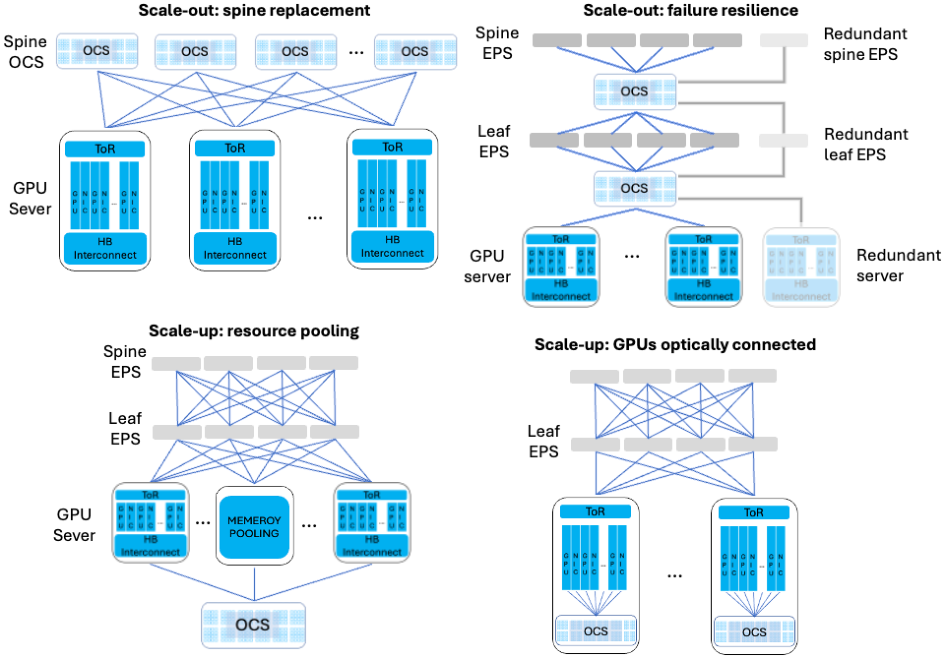
\includegraphics{figures/ch1-ocs-applications.pdf}
    \end{center}
    \caption{Optical circuit switch application in scale-out and scale-up network.
    }\label{fig:ch1-ocs-apps}
\end{figure}
% Silicon Photonic 
While industry deployments by companies such as Google and NVIDIA have demonstrated the feasibility of optical circuit switching (OCS), most existing systems rely on Micro-Electro-Mechanical Systems (MEMS) to steer light.
MEMS switches, which use tiny movable mirrors, provide reliable and low-loss optical paths, but they face intrinsic limitations for next-generation AI data centers.
Their mechanical nature imposes millisecond-scale switching speeds, and the devices are physically bulky, often requiring dedicated chassis.
Such characteristics constrain the ability to respond to the highly dynamic, latency-sensitive traffic patterns typical of large-scale AI workloads.
Silicon photonics (SiPh) addresses these limitations by leveraging CMOS-compatible fabrication to integrate complex optical functions onto a single silicon chip.
Unlike MEMS, SiPh-based switches employ arrays of integrated components such as Mach-Zehnder interferometers or micro-ring resonators, enabling reconfiguration of optical paths in microseconds.
This speed allows the optical fabric to be treated as a dynamic resource, capable of adapting to real-time traffic demands during AI model training.
In addition, the high integration density achievable with SiPh dramatically reduces the physical footprint of OCS devices, supporting co-packaged optics where switches reside within the same package as GPUs or CPUs, thereby minimizing signal loss and power consumption associated with long electrical traces.
Finally, SiPh benefits from the scalability and cost advantages of standard silicon wafer fabrication, while offering structural robustness.
Being solid-state, these devices are less susceptible to mechanical wear or environmental vibrations compared to MEMS, making them more reliable in the high-temperature, high-vibration environments typical of modern AI racks.

\subsection*{Challenges} \label{sec:challenges}
Despite the advantages of silicon photonics for optical circuit switching, deploying large-scale SiPh-based switches in hyperscale AI data centers still face complexity that has not yet to be fully addresses.
While small-scale switches have been proven, scaling these systems to meet industrial demands introduces fundamental challenges that necessitate new research.
First, high-radix scaling and architecture design present significant difficulties. Supporting modern clusters may require switches with 128x128 or 256x256 ports, involving tens of thousands of integrated actuator on a single chip.
At this density, cumulative insertion loss and crosstalk become substantial, and conventional circuit topologies are insufficient. Designing these systems demands a careful balance between port count, signal integrity, physical footprint, etc,.
The most critical operational bottleneck, however, is the large-scale control and configuration of these actuators.
In a high-radix switch matrix, establishing a data path or reconfiguring the entire network fabric requires the precise coordination of thousands of integrated actuators.
Because AI traffic patterns are highly dynamic, the traditional "one-by-one" sequential configuration of actuators is far too slow and operationally impractical.
There is an urgent need for an automated control application capable of rapid, parallelized programming of the switch matrix.
Without a software-defined tool to instantly map logical interconnect requests into hardware states, the potential for microsecond switching remains locked behind the inability to manage the hardware's complexity in real-time.
Finally, a major gap exists in System-Level SDN Integration. Currently, AI networking stacks are optimized for electronic packet switching, leaving Layer-1 optical resources without a standardized management interface.
Integrating OCS into existing data centers requires a robust Software-Defined Networking (SDN) framework that can translate high-level application demands into specific optical configurations.
This controller plane must be protocol-aware and capable of managing optical resources as a transparent, programmable layer of the overall cluster.

\subsection*{Objectives}
Considering the critical role of reconfigurable photonic integrated circuits (PICs) in scaling AI data center interconnects, this thesis is framed around the development of a comprehensive, software-defined ecosystem for large-scale optical circuit switching.
The primary aim is to establish a vertically integrated technology stack that spans architectural design, physical-layer circuit synthesis, and system-level control, thereby enabling programmable photonic processors to be seamlessly integrated into modern AI infrastructures.
Specifically, the global objective of this thesis is to contribute to the development of a scalable and manageable OCS solution that can ultimately be deployed in data center interconnects.
This project begins with the development of a graph-based programming framework to automate the synthesis and mapping of photonic circuits, bridging the gap between high-level logic and physical actuator configurations.
It then investigates scalable OCS architectures, aiming to resolve the trade-offs between port count and signal integrity.
This includes conducting in-depth blocking analysis and physical-layer simulations to evaluate insertion loss (IL) and signal-to-noise ratio (SNR) in data center environments.
Finally, an integrated gNMI-based control system is implemented for Layer-1 OCS, enabling standardized, software-defined reconfiguration and management within AI data center networks.

\subsection*{Structure of the thesis}
The thesis is organized to offer a comprehensive account of the theoretical background, methodological developments, and experimental validation associated with the research contributions.
The remainder of this document is structured into the following chapters:

\begin{itemize}
    \item Chapter 1: \nameref{chap:intro} This chapter provides the the research background and motivation, focusing on the transition from traditional electronic interconnects to integrated photonic switching.
          It reviews the architecture of modern AI data centers and highlights the increasing demand for scalable for optical circuit switching. The chapter then defines the research objectives and outlines
          the main contributions of the thesis, providing an overview of the structure of the subsequent chapters.
    \item Chapter 2: \nameref{chap:fundamentals} This chapter presents the theoretical foundations for photonic integrated circuits.
          It introduces key photonic components and circuit topologies, then develops a graph-theory-based framework for circuit modeling and routing, which enables automated control and programming at the photonic layer.
          It also outlines Software-Defined Networking (SDN) principles to support the design of an SDN-based control layer for integrating optical circuit switching into data center networks.
    \item Chapter 3: \nameref{chap:applications_on_pip} This chapter demonstrates optical networking applications implemented on hexagonal programmable photonic processors.
          By applying graph-theory-based routing algorithms, the work replaces manual and sequential tuning procedures with automated programming methods.
          The chapter presents implementations of optical interconnects, circuit switching, and multicasting functions, followed by a systematic evaluation of performance metrics.
    \item Chapter 4: \nameref{chap:ocs_archs}} This chapter develops a graph-theory-based modeling and benchmarking framework for high-radix silicon photonic switch architectures, including Benes, Dilated Benes, and PILOSS topologies.
          It analyzes hardware complexity and optical performance by evaluating metrics such as component count, insertion loss, and signal-to-noise ratio.
          Blocking probability under different routing strategies is also investigated. The chapter provides design guidelines for scalable and efficient optical switching fabrics suitable for data center applications.
    \item Chapter 5: \nameref{chap:sdn_for_ocs} This chapter presents the experimental demonstration of a silicon photonic switch managed via a gNMI-controlled in SDN.
          It introduces a custom YANG model designed to minimize control overhead while optimizing hardware performance across diverse connection types.
          The chapter validates the operational flow, showcasing near zero insertion loss through integrated SOA compensation and exceptionally low crosstalk,
          establishing a standardized pathway for integrating OCS into AI infrastructures.
    \item Chapter 6: \nameref{chap:discussion_and_conclusions} The final chapter synthesizes the research findings, discussing critical challenges such as scalability, optical losses, and the maturity of reconfigurable topologies for industrial use cases.
          It addresses the ongoing efforts toward SDN standardization and the current gaps in AI network optimization software. Finally, the chapter outlines the necessary developments for the commercialization and large-scale deployment of optical circuit switching systems.
\end{itemize}

At the end of the thesis, a section is provided with a complete list of the Author's merits and contributions to scientific journals and conferences.